% Preamble
\documentclass[11pt]{report}

% Packages
\usepackage[english]{babel}
\usepackage[indent=20pt]{parskip}
\usepackage{graphicx}
\usepackage{hyperref}
\usepackage{tabularx}
\usepackage{siunitx}
\usepackage{wrapfig}
\usepackage{tikz}

% textidote: ignore begin
\hypersetup{pdfborder=0 0 0}

\usetikzlibrary{shapes.geometric, arrows}

\tikzstyle{startstop} = [rectangle, rounded corners, minimum width=3cm, minimum height=1cm,text centered, draw=black, fill=red!30]
\tikzstyle{io} = [trapezium, trapezium left angle=80, trapezium right angle=100, minimum width=3cm, minimum height=1cm, text centered, text width=3cm, draw=black, fill=blue!30]
\tikzstyle{process} = [rectangle, minimum width=3cm, minimum height=1cm, text centered, text width=3cm, draw=black, fill=orange!30]
\tikzstyle{decision} = [diamond, minimum width=3cm, minimum height=3cm, text centered, draw=black, fill=green!30]
\tikzstyle{function} = [circle, minimum width=2cm, minimum height=2cm, text centered, draw=black, fill=yellow!30]
\tikzstyle{arrow} = [thick,->,>=stealth]
% textidote: ignore end

% Document
\title{P1}
\author{Group 4}

\begin{document}
    \maketitle

    % textidote: ignore begin
    \tableofcontents
    % textidote: ignore end

    % TODO Add introduction text for chapter here, make it much longer and remove TeXtidote ignore annotation
% textidote: ignore begin
\chapter{Problem analysis}\label{ch:problem-analysis}
% textidote: ignore end

\section{What is the problem?}\label{sec:what-is-the-problem?}

Commuting is a ubiquitous and integral part of modern life, affecting millions of people daily as they travel between
their residences and workplaces, educational institutions, or other destinations.
The objective is to delve into the issue of commuting, encompassing the issue's existence, its potential consequences,
the current perceptions of commuting, and the necessity to define the subject and purpose of addressing this issue.
A crucial facet of this analysis is to illuminate the concealed costs associated with commuting, including time, money,
and its impact on the climate, empowering individuals to make informed travel decisions~\cite{alma9921355859805762}.
% TODO Find `Enda, 2011` source and append it to \cite after `alma9921355859805762`

Commuting is a universal challenge that underpins the daily lives of individuals across the globe.
The existence of this issue is deeply rooted in the challenges faced by commuters as they navigate various modes of
transportation, from personal vehicles to public transit.
This existence is compounded by the prevalent issues of traffic congestion, stress, time inefficiency, heightened
greenhouse gas emissions, and financial strain.
These problems are accentuated by the continued urbanization and centralization of job opportunities.
As our cities expand, more individuals are drawn to urban centers in search of employment opportunities, resulting in a
growing commuting dilemma.
% TODO Find `Enda, 2011` source and insert it after `dilemma` and before `.`
The consequences of unaddressed commuting issues are multifaceted and profoundly impactful, affecting individuals,
society, and the environment.
Traffic congestion, particularly in urban areas during peak hours, results in reduced productivity, increased fuel
consumption, and growing frustration among commuters.
Extended commutes also lead to stress, anxiety, and various health-related issues, including cardiovascular ailments,
adding to the health burden.
The time spent in daily commutes consumes significant portions of daily life, diverting valuable time from work,
leisure, and personal activities.
Moreover, the reliance on personal vehicles intensifies air pollution and contributes to the pressing challenge of
climate change, raising ecological concerns.
The financial burden of commuting, encompassing expenses such as fuel, vehicle maintenance, public transportation fares,
and parking fees, places individuals and families under considerable financial strain~\cite{alma9921355859805762}.
The contemporary perspective on commuting portrays it as an indispensable yet frequently challenging facet of urban
life.
Individuals, including university students, often navigate their daily commutes through a combination of personal cars,
public transportation, cycling, and walking.
This experience is characterized by crowded public transit, traffic congestion, and a perpetual struggle to manage time
effectively.
The daily rigors of commuting frequently lead to physical and mental exhaustion, even in the face of technological
advancements and urban planning.
% TODO Find `Enda, 2011` source and insert it after `planning` and before `.`
If we focus on the issue of commuting, particularly in urban and suburban settings, as well as its implications for
university students.
It encompasses various transportation modes, including personal vehicles, public transit, cycling, and walking.
Additionally, it scrutinizes the societal and individual impacts of commuting, encompassing both positive and negative
aspects.
This subject holds relevance for students who must manage their academic pursuits alongside their daily commutes~\cite{alma9921355859805762}.
The purpose of this analysis is to raise awareness about the profound impact of commuting on individuals, society, and
the environment, with a specific emphasis on the implications for students.
By shedding light on the concealed costs of commuting, which include time, money, and climate effects, the analysis aims
to empower students and individuals to make well-informed decisions regarding their daily travel routines.
Furthermore, it underscores the necessity for innovative solutions and policy changes to mitigate negative consequences
and promote sustainable and efficient transportation options that can make the lives of university students and working
professionals more manageable.
% TODO Find `Enda, 2011` source and insert it after `manageable` and before `.`
Often the average individual, frequently underestimate the concealed costs associated with their daily journeys:

\begin{itemize}
    \item \textbf{Time}: Commuting consumes a substantial portion of daily life that could be more productively
    allocated to work, leisure, or personal activities, thus influencing students' academic and personal lives.
    \item \textbf{Money}: The expenses associated with commuting, including fuel, maintenance, parking fees, and public
    transportation fares, accumulate over time and impact individuals' financial stability, an issue that particularly
    affects students managing their budgets.
    \item \textbf{Climate Impact}: Commuting contributes to carbon emissions and air pollution, exacerbating
    environmental challenges, and underscores the significance of environmentally conscious transportation choices that
    resonate with students~\cite{alma9921355859805762}.
\end{itemize}

Commuting is a pervasive issue that significantly influences the daily lives of people, particularly university
students.
The consequences of unaddressed commuting problems encompass physical and mental health challenges, financial burdens,
and environmental impacts.
Current perceptions of commuting highlight its necessity but also the challenges it poses.
By making individuals aware of the hidden costs of commuting, such as time, money, and its environmental impact, this
analysis aims to empower individuals, especially students, to make more informed travel decisions.
Moreover, it emphasizes the need for innovative solutions and policy changes to mitigate negative consequences and
promote sustainable and efficient transportation options.
In doing so, it seeks to improve the quality of life for students and the broader population while addressing pressing
environmental concerns.

\section{Make people aware of how much commuting costs}
\label{sec:make-people-aware-of-how-much-money-time-climate-they-are-using-on-commuting}

This section will focus on the aforementioned concealed costs of commuting, which are time, money, and climate and
health effects.
A study from Denmark’s statistic clearly shows that out of the around three million people in the workforce only
185 thousand people don't commute to work~\cite{erhvervspendling2021}.
This means that \(93.88\,\%\) of the working population commutes to work in Denmark.
The full table can be seen in Figure~\ref{fig:dst-commute}.

\begin{figure}
    \centering
    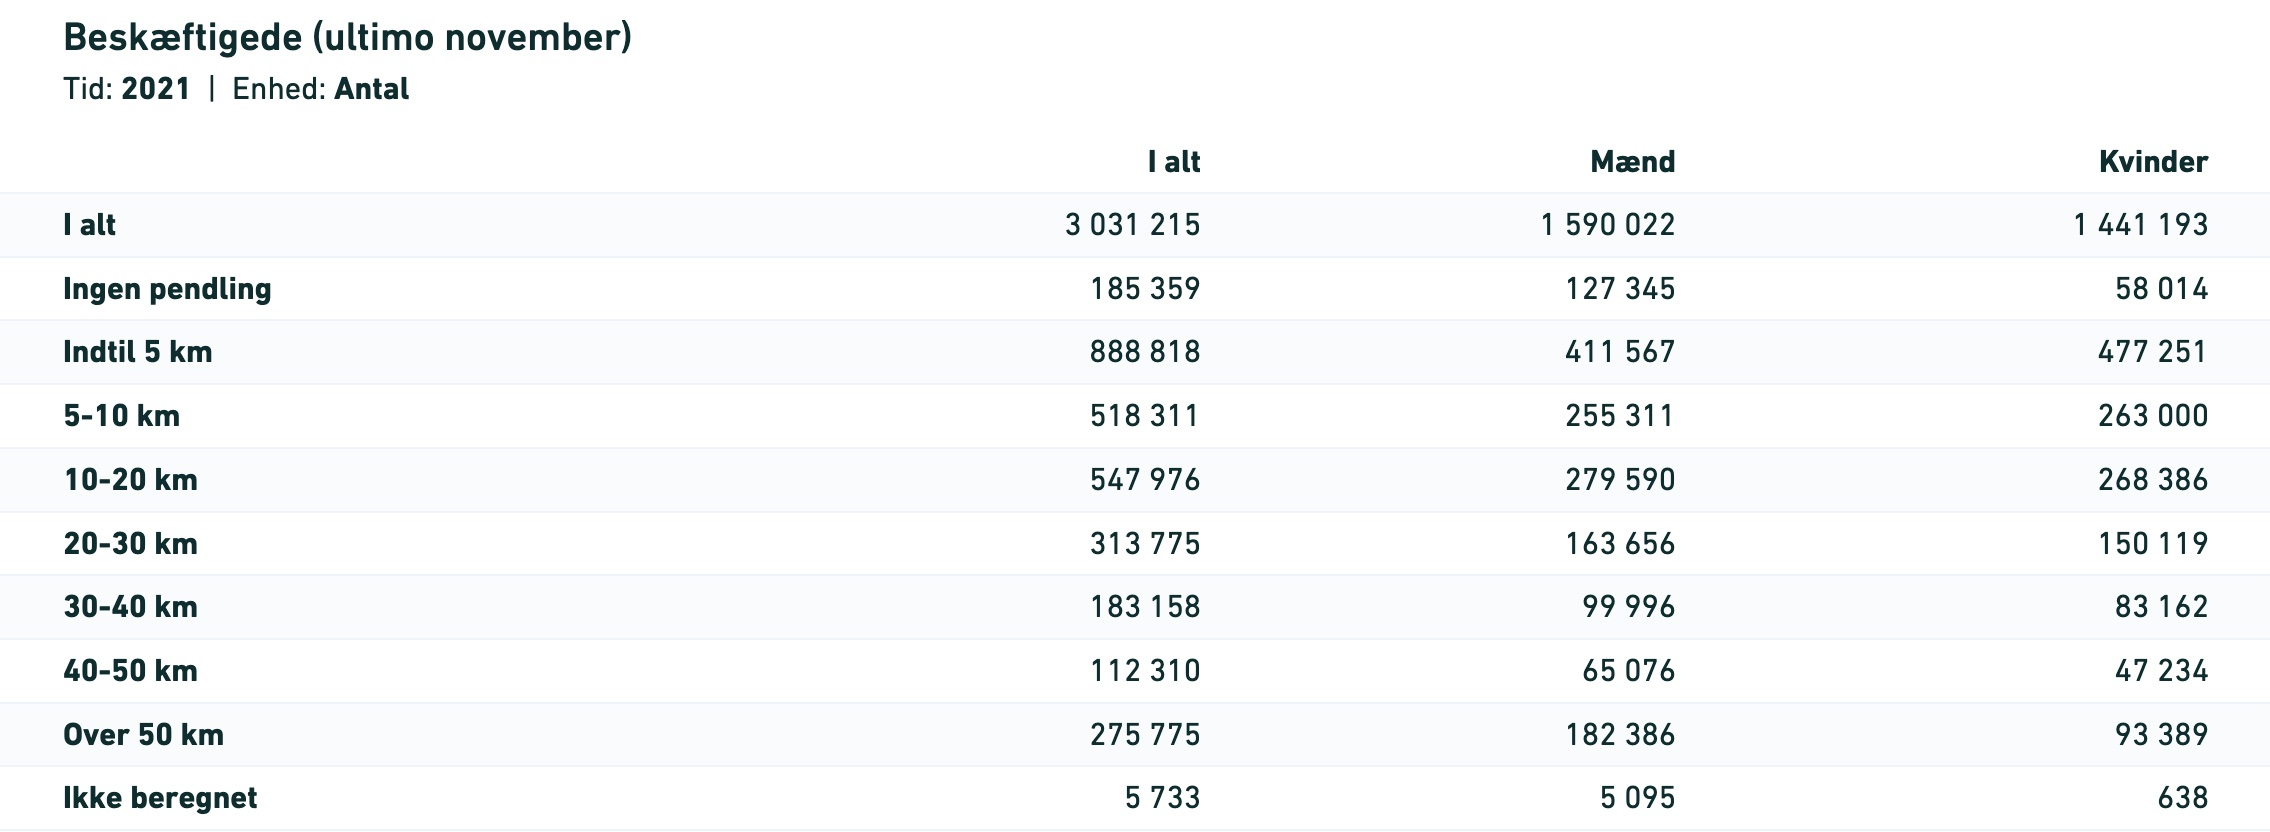
\includegraphics[width=\textwidth]{stats}
    \caption{Amount of people that commute by distance~\cite{erhvervspendling2021}.}
    \label{fig:dst-commute}
\end{figure}

\subsection{Time Cost}\label{subsec:time-cost}

Commuting takes time, and that time can increase depending on the distance of the travel or by transportation choice.
Why the time spent commuting is important is because it can have an effect on the quality of life.
A Chinese article looked into the effects that longer commuting have on our lives~\cite{commuting-time2022}.
They highlight how longer commuting results in lower the satisfaction with work and life.
Longer commute can also have an effect on the physical body, as the user stays inactive for long periods of time.

They also mention how many would choose to change their residence or workplace to decrease the time spent commuting.
Many people are thus faced with the choice of either commuting longer or changing their residence or workplace.
Both of which have their advantages and disadvantages.
Longer commute has the disadvantages mentioned above, while changing residence or workplace can be difficult and
stressful.
That is a choice that the user has to make for themselves, but it is important that they are aware of the consequences
of their choice.

\subsection{Financial Cost}\label{subsec:financial-cost}

Another critical aspect is how commuting effect the economy of people.
A study shows that the average American citizen spends \SI{8466}[\$]{} on commute expenses~\cite{bankrate2023}.
There is a different cost involved in the commute depending on which transport options are used.
For example, \(76\,\%\) of commuters use their personal vehicle~\cite{bankrate2023}.
They may also have some extra expenses besides just the buying price of the car.
The average driver spends \SI{1771}[\$]{} on full car insurance and furthermore they spend money on car maintenance
and occasionally after 5000 miles they need to get their vehicles' oil changed.
This could be a challenge as research shows that 1 out of 3 drivers can't afford sudden unexpected car repairs.
The study also suggests that using public transport, bike or scooter to work will cost less~\cite{bankrate2023}.
This change could be difficult as commuting in a personal vehicle could be much more time efficient.

The same study showed that the working poor who commuted by public transport spend \(10\,\%\) of their income on
commuting compared to \(21\,\%\) when commuting in their car.
The working poor prefer saving money because this means they can spend a larger portion of their income on other
relevant expenses like food, healthcare, household supplies and saving for the future.
From this, it is apparent that especially the poorer people would prefer having the opportunity to
commute by cost preferences.
This could improve their economy as the working poor tend to use the least expensive options of commuting, like
carpooling, van pooling, biking, walking and public transport.
Comparing this to people with higher income they are more inclined to spend more on commuting~\cite{bankrate2023}.

\subsection{Climate Effect}\label{subsec:climate-effect}

People are generally uninformed about how much emissions they are helping to produce while travelling in their
desired commuting option.
The desired preference of the commuting can change the way people commutes.
A study made in 2021 on commuting showed which transport option users would pick depending on what their preferences
were.
In this study, we can clearly see that public transport is preferred when the priority is saving time, cost or being
environmentally friendly while walking or cycling were more preferred when health was the priority~\cite{spark2023}.

This is interesting because if people had the opportunity to select either economy, time or sustainability as a
preference when commuting they could use alternative transport options.
Furthermore, this could possibly promote sustainable commuting.
This may be important as sustainable living is becoming more trending than ever, which may also be a direct result of
people becoming more aware of how their choices can have an effect on the environment they live in.

Research done by the Capgemini Research Institute shows a correlation between sustainability and significant business
benefits.
This means that customer loyalty and revenue increases by having a focus on being sustainable~\cite{capgemini2020}.
The enlarged focus on sustainability stems from the new youth, as they prioritize sustainability more than millennials.

\subsection{Health Effect}\label{subsec:health-effect}

Commuting can also influence mental health and well-being as it can cause an increase in stress level.
One study suggests that one of the factors increasing stress levels is that the commuters have a difficulty in
appreciating their way of commuting~\cite{koslowsky2013}.

The author furthermore explains that the governments must prioritize what the commuters prefer.
These workers can have an incline in stress levels as they have deadlines and specific meeting times that need to be
reached in time~\cite{koslowsky2013}.
By this we can derive that having the opportunity to travel to your destination as fast as possible can be beneficial
for the health.
We look further into the health effects of commuting in~\ref{sec:health-consequences}.

Another study on 208 people who were rail commuters in New York showed that the longer time that they commuted the more
their cortisol level increased~\cite{commuting-health2006}.
This means that time duration of commuting is an important factor for some users.
Therefore, it is essential that people commuting can have an influence on time spent commuting.

\section{The history of commuting}\label{sec:the-history-of-commuting}

The problem of choosing public commuting, private commuting or moving closer to one's place of work is a more modern
problem.
People have been commuting since the beginning of humanity - from fetching berries in the forest to traveling to
fighting in wars.
In more recent human history commuting encapsulates something more complex.
Before the information age in the 20th century and before cars and buses and such were mainstream transport vehicles,
most people traveled on foot or were accompanied by some animal suited for travel to and from work.
This trend reversed as cars and other more technologically advanced vehicles became accessible.
In the early 19 hundred Netherlands, as described in the book ``No bicycle, No bus, No job'', people would flock to the
cities to avoid unemployment as the industrial evolution was in full force.
As most workers were from a lower socioeconomic class with limited resources to spend on transport and luxury, it only
made sense for workers to move closer to the factory they worked at to save time and money~\cite{bek2022}.

\subsection{Technological breakthroughs}\label{subsec:technological-breakthroughs}

As the Netherlands, as well as most other European countries, experienced the same technological breakthroughs in the
same relative timeframes in history, the country is in broad sense comparable to Denmark.
As cars and buses and such populated the streets in the 19 hundreds, commuting slowly became the complex issue we
know it as today.
The escalation of the big cities throughout the 20th century also brought higher education for the people.
The number of people completing higher education in the last 50 years is considerably higher than it was in the
beginning of the 20th century as seen in Figure \ref{fig:figure5}.

\begin{figure}
    \centering
    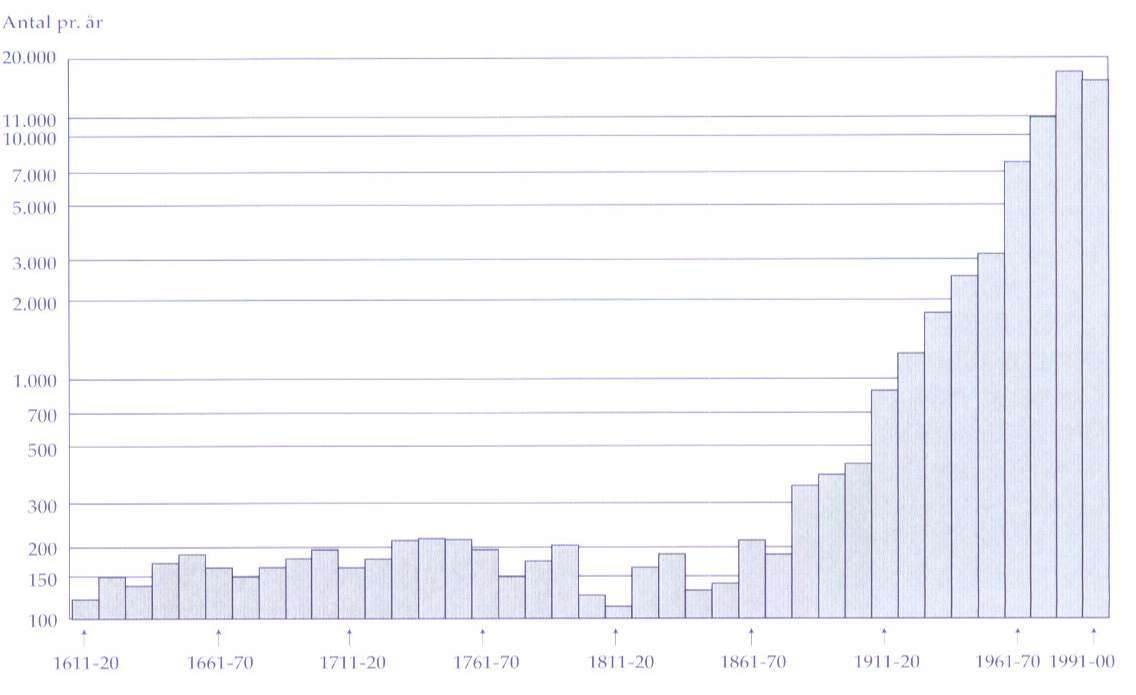
\includegraphics[width=\textwidth]{images/education-levels}
    \caption{Historical education levels in Denmark~\cite{johansen2005}.}
    \label{fig:figure5}
\end{figure}

This trend of higher education played a part in the acceleration of technological advancement in society, improving
quality of life of the working class.
With this improvement, more money became available to the working and upper class.
Even though quality of life has improved consistently, the Gini coefficient in Denmark has risen 7.7 percentage points
since 1987~\cite{cepos2023}.
This development has played a significant role in the lack of affordable housing and living in the big cities forcing
working class people to move out of the cities they work in to be able to afford stable housing.
As the big cities still need unskilled and skilled workers in its facilities, the problem of the commute arises.

Commuting in the rural areas of the country is heavily influenced by cars, as the population density is dramatically
lower there compared to in the big cities~\cite{mulacic2020}.
As a comparison, the present Copenhagen region encapsulates 35\% of the
population while only occupying 7\% of the land area in Denmark~\cite{nielsen&lemberg2017}.
This results in heavy reliance on public transport in big cities, as roads are not big enough for everyone to drive a
car to work every day as opposed to less populated areas where the roads have the capacity for everyone to commute via
car.

\subsection{The history of public transport in Copenhagen region}
\label{subsec:the-history-of-public-transport-in-copenhagen-region}

Public transport is therefore a part of the equation when it comes to the commuters' preference.
This has not always been the case, as public transport in the 19 hundreds was lackluster, unreliable and scarce.
The working norm, after the industrial revolution had officially settled into society, was very much controlled by the
factory owners, who demanded specific working hours for their employees.
This resulted in congestion when arriving at work and similar congestion when going home again~\cite{bek2022}.

In today's day, many sectors and businesses have different working hours.
Some are set in stone for obvious reasons, such as hospitals.
Others such as office workers and other officers are just required to work 7 to 8 hours of work per day, regardless of
when this work is performed.
Some jobs are even possible to do from home due to the internet and technological advancements.
This evolution of this work environment in history has made it possible for a worker to work in the city, while living
in the suburbs through commuting or working from home.
All these scenarios, whether you are living in the city or in the suburbs, and whether you are working in the city or
in the suburbs it needs to be encapsulated into our program to properly include every scenario and thereby expanding the
use cases of our program.

\section{Target audience analysis}\label{sec:target-audience-analysis}

When working on a large scale project, it is important to analyze who the target user-base is.
The problem has to be big enough to affect numerous users and the solution has to be viable to be used by said
users.

\subsection{Users}\label{subsec:users}

The main issue is about travelling, which covers a wide range of people, as almost everyone travels one way or
another.
Some examples include travelling to work, travelling to school, family visits, or outings with friends.
As this range is too broad we will in the following section narrow the target user-base down.
There are already some solution to this issue, but in Section~\ref{sec:extant-solutions-and-their-operational-mechanisms},
we figured that these already existing solutions are more fit for single trips, rather than every day travelling.
This gap in use case is mainly what we want to focus on, which is why our target audience is \underline{commuters}.

\subsection{Age range}\label{subsec:age-range}

With our user group in mind, we can estimate an age range for commuters.
Commuting means to travel to the same destination and back on a regular basis.
Therefore, our focus on destinations for commuting are either education or work.

In Denmark, primary schools are chosen for students based on the district where the student lives~\cite{primary_school}.
This would exclude them from our target user-base, as we want to focus mostly on long distance commuters.
At shorter distances, we would need to exclude planes, trains, and for people younger than 18, cars, making it a matter
of whether the student should commute by walking or by bike, which are both \unit{CO_{2}} friendly options and trivial
to select between, making our solution somewhat irrelevant for this age group.

From secondary education however, students can freely pick which high school they want to go to and the closest school
will be assigned to them.
This, however, makes them a candidate for our user-base, as there are not as many high schools as there are primary.
Many students therefore have a longer commute to school.
Secondary education starts when the student is 16 years old~\cite{secondary_school}.
Our cutoff in the age range would be retirement, as we assume that retired individuals will no longer be commuting in
retirement.
The retirement age in Denmark is 66-68 years of age~\cite{retirement}, making our age range
\underline{between 16 and 68 years}.

The age range is rather large as the user-base includes a large part of the population, which makes our solution rather
difficult, as we have to accommodate it for teenagers as well as adults and the elderly.
The program will therefore have to tailored to all these age groups.

\subsection{Persona}\label{subsec:persona}

To further analyze our user-base, we decided to use the \textit{persona} method.
It works by creating fictional people with different fictional issues and look into how our solution could help them
with their issue.
Below are three personas, with their images generated by GAN AI~\cite{thispersondoesnotexist}, where each of them
cover different age groups and have distinct characteristics related to the main problem.

\renewcommand{\arraystretch}{1.5}

\noindent
\begin{tabularx}{\textwidth}{ | l X | }
    \hline
    &                                               \\
    & 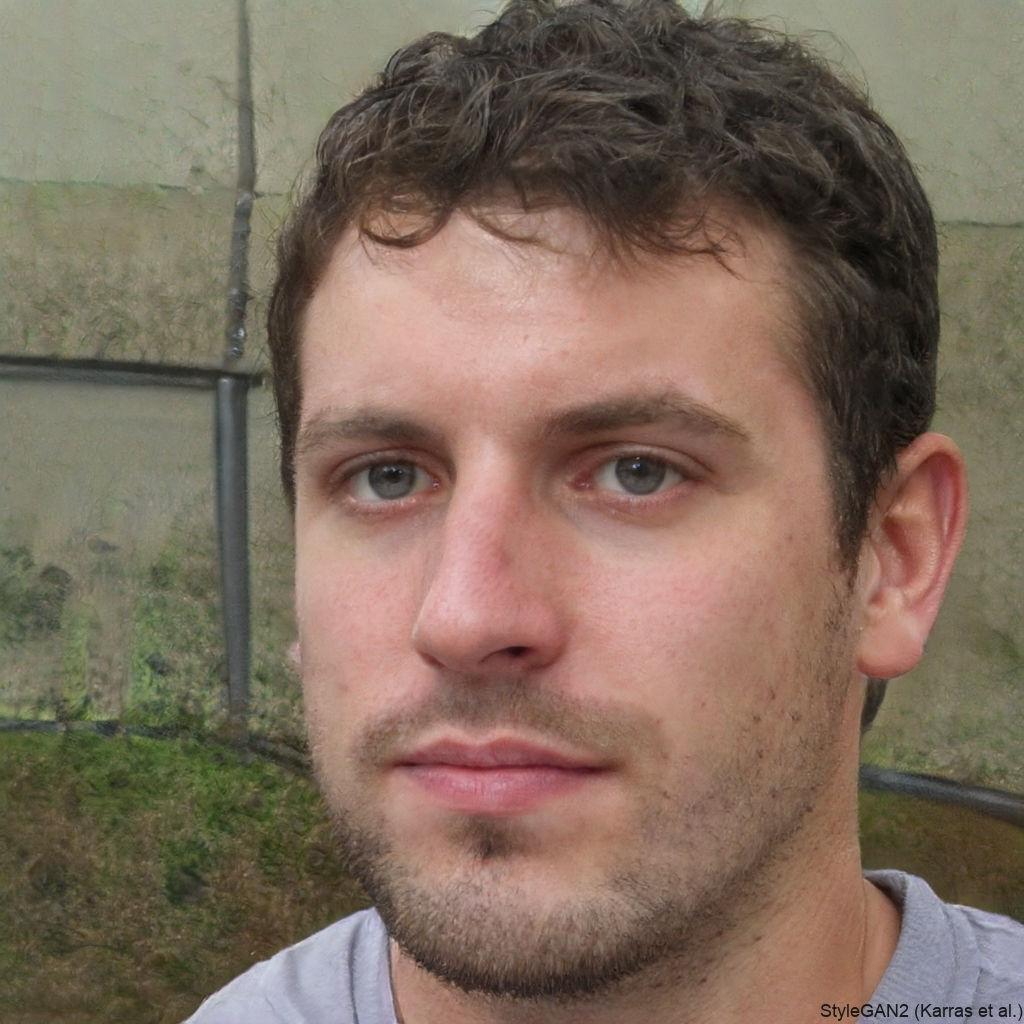
\includegraphics[width=0.25\textwidth]{asger} \\
    Name       & Asger Johansen                                \\
    Age        & 28 years old                                  \\
    Occupation & Designer                                      \\
    What's important & For Asger it is important to spend his days to the fullest.
    He is very outgoing, so he goes out with people after work.
    He hates having to stay overtime. \\
    Current problem & Asger just got a new job offer, but it's in another city.
    He isn't sure whether to move out or to commute there.
    He is also afraid of losing his free time if he has to travel. \\
    Potential solution & We would want to make a program, where Asger could calculate how long it'd take to commute from
    where he lives to the new job.
    He could compare different forms of transport and decide whether it's worth it to commute or if he should move out
    instead. \\
    \hline
\end{tabularx}

\noindent
\begin{tabularx}{\textwidth}{ | l X | }
    \hline
    &                                                  \\
    & 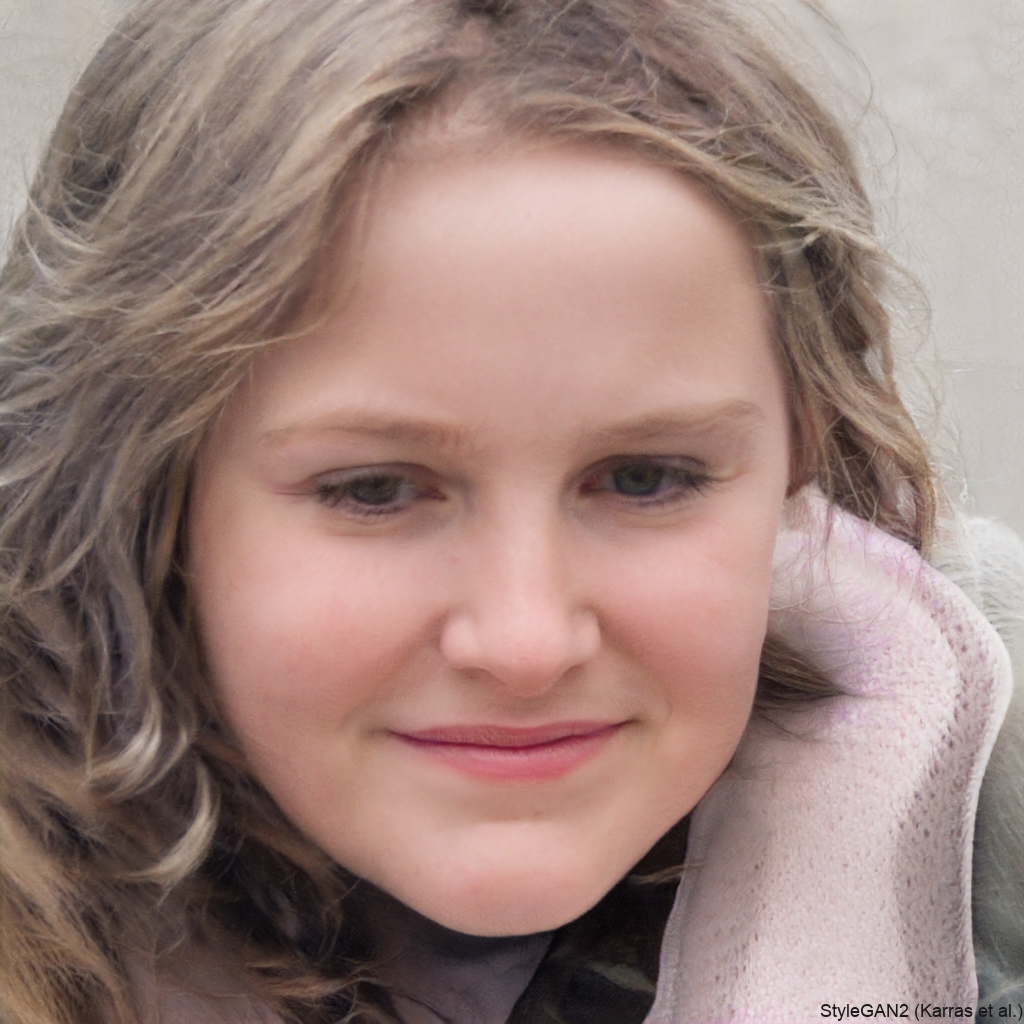
\includegraphics[width=0.25\textwidth]{josefine} \\
    Name       & Josefine Madsen                                  \\
    Age        & 19 years old                                     \\
    Occupation & Student                                          \\
    What's important & For Josefine it is important to look after the nature.
    She's been taught to think green since she was little, so she doesn't like taking public transport and doesn't want
    to drive a gas car. \\
    Current problem & Josefine is starting university, but she lives outside the city.
    She is considering whether to take the S-train, the train or a bus to university.
    She is also considering buying an electric car. \\
    Potential solution & We would want to make a program, where Josefine could calculate how much the emissions is made
    from different forms of transport.
    She can then compare them and choose what works best for her. \\
    \hline
\end{tabularx}

\noindent
\begin{tabularx}{\textwidth}{ | l X | }
    \hline
    &                                                \\
    & 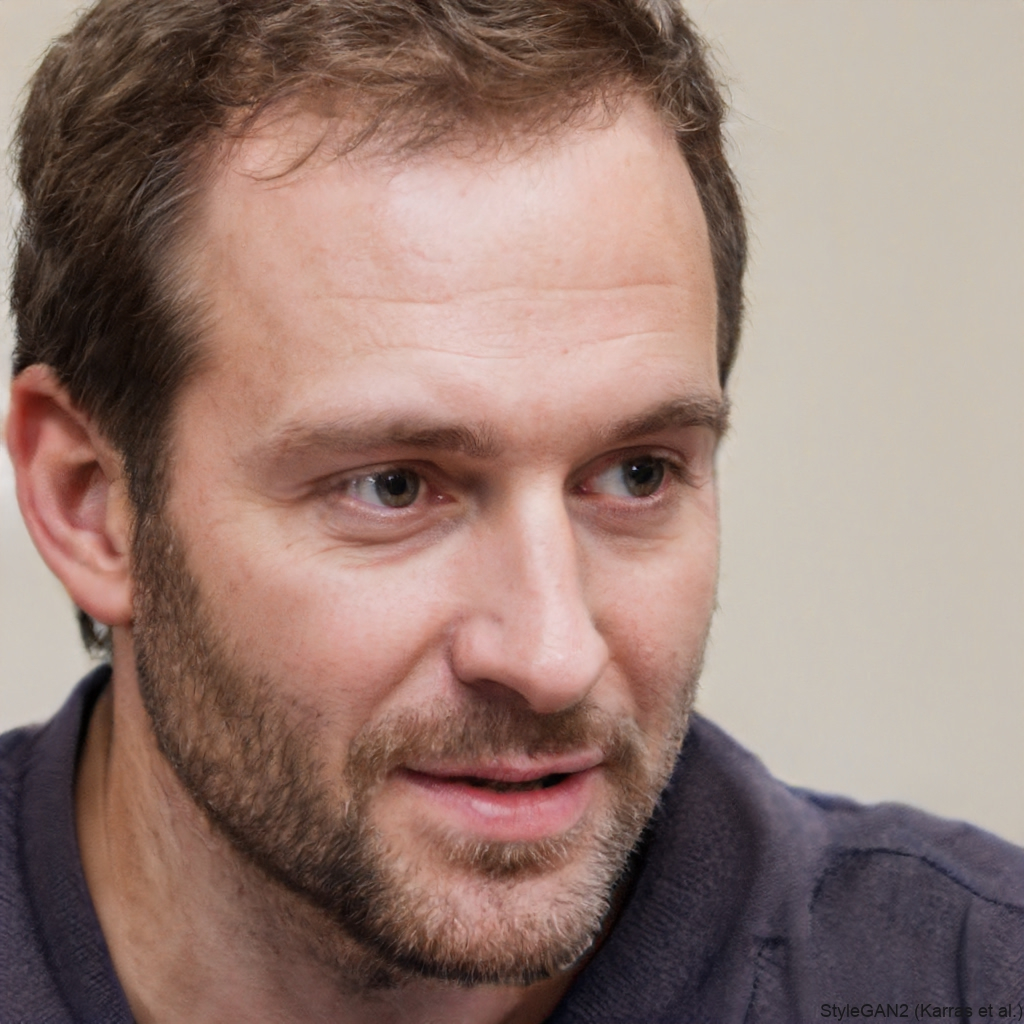
\includegraphics[width=0.25\textwidth]{martin} \\
    Name       & Martin Jensen                                  \\
    Age        & 34 years old                                   \\
    Occupation & Factory worker                                 \\
    What's important & For Martin it is important to live a carefree life.
    He has a family and friends at work, so he's pretty happy with himself. \\
    Current problem & Martin drives a gas car to work, but he wants to change that for the sake of the environment.
    He has gotten used to the comfort of his car, but can't afford an electric car.
    He wonders if public transport could match that. \\
    Potential solution & We would want to make a program, where Martin can figure out what forms of public transport are
    most comfortable and most climate friendly. \\
    \hline
\end{tabularx}

\section{Context}\label{sec:context}
Commuting is one of the staples, so to speak, of modern life, and a central part of the post-modern industrialized
society.
As cities rapidly grew after the industrial revolution and more and more large-scale workplaces became the norm in
cities, people started commuting to work from suburban areas to the city.
In the early stages of this development in the beginning and middle of the 20th century, commuting was a rather simple
task: People just had to get to work in the mornings and back home in the evenings.
Nowadays, the complexity of commuting has increased drastically with many additional factors having to be considered,
e.g., how big of a carbon footprint is acceptable for me?
This question especially became relevant in recent times due to the increasingly noticeable effects of climate change
and the scientific evidence that increased CO2 emissions greatly contribute to climate change.
Other questions the modern-day commuter might ask themselves are: Do I need/want to commute every day, or is it ok if I
work from home part of the week?
What should be the balance between cost and environmental protection?
Do I live in an area where the availability of public means of transportation is scarce, so I am more inclined to use a
car?
One of the simpler questions someone that considers commuting could ask themselves is merely: What commuting route
should I choose?
With the advent of the digital age and smartphones, the answer to this question have become commuting planner
applications, that have become increasingly popular in recent years, helping individuals plan their daily commutes
efficiently and minimize travel-related stress.
These applications offer various features and functionalities, but they often have shortcomings that prevent the
commuter from more advanced planning strategies, including the lack of easy access to cost and environmental impact
information, e.g., how much C02 will be spent on a trip, how much a trip will cost, as well as limited user control over
how these factors are weighed in route calculations.
Existing solutions include the (mostly) worldwide available Google Maps, the popular Danish Rejseplanen service and a
couple of other mobile and web applications that are not location-bound but can be used internationally, like
\url{commute.org}.
We will now look at some existing solutions and discuss their shortcomings to better understand the root of the problem.

\subsection{Google Maps}\label{subsec:google-maps}
The above-mentioned application is a widely used travel and commuting planner that provides detailed navigation and
route information.
While it offers estimated travel time and distance, it lacks a direct and user-friendly way to determine the cost of the
trip or the CO2 footprint.
Users cannot easily access information about how much money the trip will cost, as Google Maps does not integrate with
financial or payment apps to calculate expenses like tolls, fuel, or public transportation fees.
This makes sense since Google tries to target a large international audience with the application, making is difficult
or nearly impossible to cover every localized payment solution or traveling restriction.
Similarly, it does not provide real-time data on the CO2 emissions associated with the chosen route, making it
challenging for users to make informed decisions about their environmental impact.
Users have very limited control over how cost and environmental factors are weighed in route calculations, as Google
Maps primarily focuses on travel time and distance.
The only available selection options are preferences for means of transportation and whether the route should be
calculated with ``fewer transfers'', ``less walking'' or ``wheelchair accessible'', where all three of the options
seem to be tailored towards people with restricted mobility.

\subsection{Rejseplanen}\label{subsec:rejseplanen}
In Denmark, the most popular commuting planner application by far is Rejseplanen.
This application, just like Google Maps, is both available as a web and mobile application.
The app lets the traveler or commuter to enter trip starting and ending locations, which it then uses to calculate a
route using public means of transportation or as secondary options as walking routes.
When a route is calculated, the user is presented with a list-like interface from which the details of the trip can be
read; what means of transportation will be used, which lines, what the departure and arrival times are, and if there are
any special restrictions on the trip.
Getting the price of the trip is possible too, but in a primitive manner that doesn't consider factors such as if the
user is a tourist or a regular resident, which is an important feature since tourists might have different traveling
strategies than regular residents, and additionally tourists might not use the prepaid Rejsekort card, etc.
There is an additional option of adding your Rejsekort ID to the app, so it can calculate the trip price based on your
card plan, but even that feature is kept rather simple, possibly because the Danish transportation authorities also
released the DOT app, whose primary responsibility is exactly that: calculating trip prices and buying tickets.
The user can also customize the trip’s parameters slightly, e.g., if it’s a biking or a walking trip, what the maximum
allowed biking or walking distance should be, whether the user is a “slow”, “medium” or “fast” walker (even though there
is no guideline for how fast exactly each of these options is), and a few additional details, but a feature that
definitely lacks is the calculation of the trip’s total CO2 emissions, which is an important factor in the modern-day
world.

% textidote: ignore begin
\section{Health consequences}\label{sec:health-consequences}
% textidote: ignore end

% textidote: ignore begin
\subsection{Commutings effect on relationships}\label{subsec:commutings-effect-on-relationships}
% textidote: ignore end

Another aspect of the commute is the health benefits and consequences of different types of transportation.
The long commute has other health effects than physical ones - it also affects relationships.

Long commuting couples has a higher risk of separation compared to shorter commuting ones~\cite{sandow2011}.
This makes sense, as commuting takes up valuable time couples could have been spending together, which in turn could
have strengthened their relationships.
Along with the increased rates of stress-related symptoms when commuting, couples have a harder time staying together
and focusing on each other rather than on the contents of the commute.

Even more concerning is that men in couples that commute on a temporary basis experience the highest risk of separation.
Also, women experience less risk of separation when commuting for a longer time period.
These risks also depend on where the couple resides~\cite{sandow2011}.
These separation risk theories take into consideration that the commute has to be at least 30 kilometers long.
This also makes sense, as the sporadic nature of switching one's habits, such as commuting patterns, in one's household
can have a negative effect in the same way other sporadic events can severely change the dynamic of the relationship,
such as having a baby, losing a family member or getting fired.
Therefore, it is interesting for a user of our program to be able to select a maximum commuting length, as this will
probably indirectly benefit them in their relationships.




\section{Recommendation systems}\label{sec:recommendation-systems}

In Denmark when using apps to guide your travels, you will have to choose between the different means of transport such
as: by car, train, bus, cycling or walking.
If you wanted to prioritize your climate footprint with these already existing apps you would have to research how much
a specific means of transportation pollutes.
Another situation is the economics of one's travel.
Instead of individuals having to calculate for themselves how much money they would spend on a specific travel type,
it could be done automatically.
To make it as easy as possible to make an informed decision for the users of our program, we want to automate many of
these calculations, such that the users can get an overview of their situation in a fast and easy way.

To accompany this, the authors will build a system that shows the routes that the user would want to travel by based on
their personal preferences.
This can also be called a recommendation system (RS).
RS is something we all use every day, when browsing a web shop, YouTube or other streaming services.
The goal of an RS is to sort through all available data and assume and present the most useful data to the user.
The close parallel there is between these RS and our problem solution gives rise to a segment explaining RS in more
detail.

A real world example of where this is used is in a movie recommender.
Movies are somewhat easy to classify, as one can look at the genres of different movies for example.
This type of RS works by filtering the movies through genres and is called ''content based filtering'' as seen in.

\begin{figure}
    \centering
    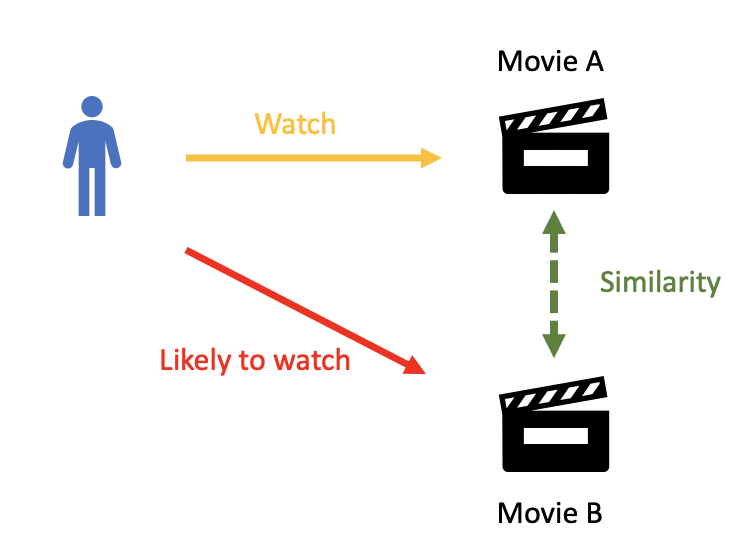
\includegraphics[width=\textwidth]{content-filtering}
    \caption{Content filtering~\cite{content_based_filtering}.}
    \label{fig:figure3}
\end{figure}

An example would be user a watching an action movie, movie A, and the system would then remember user a's preferences
and recommend another action movie, movie B, to the user as seen in ~\ref{fig:figure3}.
This is a very simplified version of content filtering as they usually utilize multiple attributes from both the content
and the user.
In the context of a movie recommender this could be both the themes, the producer, the actors etc.
In content filtering, a user's history and interactions is used to create the profile for the RS to give suggestions.
Although content filtering is better than recommending random movies, it does not take human tendency to have changing
opinions and tastes into consideration.

Another type of filtering is Collaborative filtering (CF).
CF works by comparing users with each other.
This means that CF groups users by similarities in their watched movies, and then suggests movies from the users group,
as seen in~\ref{fig:figure4}.

\begin{figure}
    \centering
    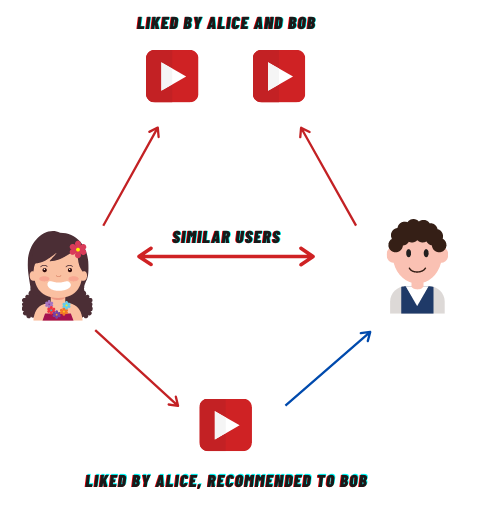
\includegraphics[width=\textwidth]{collaborative-filtering}
    \caption{Collaborative filtering~\cite{collaborative_filtering}.}
    \label{fig:figure4}
\end{figure}

Using CF does not limit the recommendations to genres or other attributes that the program already know the user
watches.
It can also recommend things from other genres, which would not have been recommended by the content filter.
Generally for both these types of filters, they need a lot of information about both the user and the content.
This is however out of the scope of this project.
While content filters and collaborative filters are versatile in their use, the goal for this project is to use them to
recommend routes and make the user aware of both the monetary impact and the impact on our climate as well as
recommending the best routes.
In this context, it would be more logical and simpler to get the users preferences directly through what could be a
questionnaire, rather than relying on behavior analysis.
The attributes one could use for the filters are straight forward, as they could be climate impact, cost, time and
others.
This would however require some analysis to get more useful data out of the routes we generate.
Using a weighted system to measure the results of our program would allow us to choose a specified amount from the top,
and by doing this we will have chosen the most relevant for the users.

\section{Summary}\label{sec:analysis-summary}

The analysis exemplifies how both the monetary cost and the concealed costs of commuting affects individuals,
as well as society.
It could be seen that price, time, environment and health all have an impact on the commuting experience.

Commuting has historically been a part of human society since ancient times, but as technological revolutions
happened with automobiles and trains urbanization began to have a stronger effect on the commuting experience.
To narrow down the scope of this paper we will choose to focus on helping commuters who need commuting for a prolonged
period of time, this could be commuting to work or for education which is something that one will need to do for
multiple years daily.
We created personas that encapsulate this target group in~\ref{subsec:persona}.
The existing solutions mainly focus on single trips some place, and are therefore focused on price and time
optimization which is not enough for repeated trips.
Through the factors that have the biggest effect on commuting, which are: price, time, environment and health.
It seems possible that a good solution to the problem would be introducing a recommendation system based on these
factors, because it would help an individual understand all the possible methods of transportation.


    % textidote: ignore begin
\chapter{Problem statement}\label{ch:problem-statement}
% textidote: ignore end

The following chapter entails the problem statement to be concluded upon.

% textidote: ignore begin
\section{Problem delineation}\label{sec:problem-delineation}
% textidote: ignore end

In contemporary society, the pursuit of employment in metropolitan areas clashes with the desire to maintain close
familial ties in hometowns.
As a result, individuals have to make the complex decision of whether commuting should be chosen as the means of
going to and from work.

The intricate considerations encompassing transportation options, time allocation between work and family, environmental
implications, and work flexibility create a challenging landscape for prospective as well as established commuters.

% textidote: ignore begin
\section{Problem statement}\label{sec:problem-statement}
% textidote: ignore end

How can we create software to help commuters select a commuting route that best suits their preferences?

% textidote: ignore begin
\section{Sub questions to problem statement}\label{sec:sub-questions-to-problem-statement}
% textidote: ignore end

% textidote: ignore begin
To answer this question, we will also be asking ourselves some sub questions that align with the overall problem
statement to conclude with a more nuanced answer.
% textidote: ignore end

\begin{itemize}
    \item What can we do to inform commuters about the environmental impact that different forms of transportation
    cause in their commuting routes?
    \item How can we help individuals make a choice on whether to move closer to their place of occupation or to commute
    from their current place of living?
\end{itemize}

    % TODO Add a lot of text to this chapter and remove TeXtidote ignore annotation around the \chapter command
% textidote: ignore begin
\chapter{Problem solution}\label{ch:problem-solution}
% textidote: ignore end

% textidote: ignore begin
\section{Motivation behind problem statement}\label{sec:motivation-behind-problem-statement}
% textidote: ignore end

We believe that the reason for these challenges is the complexity of obtaining high-quality information, thus reducing
awareness and a base for a proper decision.
By giving potential commuters an application to plan their route according to their preferences, many more would try
commuting by public transport or otherwise carbon-emission friendly options, which in turn would improve everyone's
quality of life.

This project attempts to develop a decision-support system tailored to aid individuals struggling with the choice of
commuting, aiming to integrate diverse commuting strategies into a compact and efficient application solution.

By addressing the multifaceted nature of commuting decisions, our solution seeks to optimize commuting choices,
considering cost-effectiveness, time efficiency, and environmental impact, thus assisting individuals in making
informed and balanced decisions about their commuting commitments.

\section{Software Requirements Specification}\label{sec:software-requirements-specification}
% textidote: ignore end

The outline of the requirements of the program is divided into four categories: essential requirements labeled as
``Must-haves (Mo),'' desirable requirements labeled as ``Should-haves (S),'' and ``Could-haves (Co),'' and
undesirable requirements as ``Won't-haves (W).''
The requirements are made by taking use of the MOSCOW model as it narrows our program to what is realistically
achievable~\cite{hudaib2018requirements}.
% textidote: ignore begin
``Must-haves (Mo)'' include all functions of the program that are necessary and must be included and implemented. In
contrast, ``Should-haves (S)'' and ``Could-haves (Co)'' include functions that are desirable but not critical to
the core functionality of the program.
% textidote: ignore end

The requirements are based on the personas in Figure~\ref{fig:persona_asger},~ Figure~\ref{fig:persona_josefine} and
Figure~\ref{fig:persona_martin}.

% textidote: ignore begin
\subsection{Must-haves (Mo)}\label{subsec:must-haves}
% textidote: ignore end

\begin{itemize}
    \item Evaluate user input
    \item Get requests from Rejseplanen’s API
    \item Compare routes
    \item Evaluate the weighing of routes
    \item Output calculated data based on a route to the console
\end{itemize}

% textidote: ignore begin
\subsection{Should-haves (S)}\label{subsec:should-haves}
% textidote: ignore end

\begin{itemize}
    \item Search and choose stops
    \item Use a map-related API
    \item Cross-platform compatibility
\end{itemize}

% textidote: ignore begin
\subsection{Could-haves (Co)}\label{subsec:could-haves}
% textidote: ignore end

\begin{itemize}
    \item Sort journeys by health preferences like stress or physical activity
    \item Graphical user interface (GUI)
    \item Desktop/mobile/web application
\end{itemize}
% textidote: ignore begin
\subsection{Won't-haves}\label{subsec:wont-haves}
% textidote: ignore end

\begin{itemize}
    \item Advanced security features like encryption or user authentication
    \item User health tracking or personalized health recommendations
    \item Real-time updates to a shown journey.
\end{itemize}

% textidote: ignore begin
\section{Flowchart of the program}
% textidote: ignore end

A flowchart is a diagram that describes a program's process and breaks it down step by step.
This is crucial because programming processes can often appear complex and confusing at first glance.
The flowchart shows how the program progresses through various possibilities, which helps developers to gain a much 
clearer visual overview of the program itself.
Flowcharts consist of different shapes connected by arrows.
Generally, rectangles with rounded corners are used to signal when the program starts or stops. 
Regular rectangles are used for back-end - processing and parallelograms are used for front-end - input or output. 
Diamonds are used for decisions and in our case we've made a circle to represent a function. 
This detailed process significantly contributed to our development by providing the team with clarity.

We start with an input function, which first asks the user for their current/start position and for their desired
destination.
We then give the user a choice. 
That's what makes our program special, the user can set custom preferences for the trip. 
If the user selects that, then they're asked to select what transportation they want to use. 
That can vary between cars, trains, bikes, walking and so on. 
In order to accurately calculate the \unit{CO_{2}} emissions, we require the user to enter their car's fuel efficiency. 
Then they can set priorities, which would determine what the search results are. 
Afterwards, the user has a choice to save the preferences to a file, making the process easier next time they have to
use the program.
The next couple of functions take place in the back-end.
We make calls to Rejseplanen's API, which would return the list of routes that we need.
But that's not all the information we require, therefore we make further calculations to find out what the attributes
are for all the routes. 
Then we evaluate them according to the user's preferences, assign a number to them and sort them.
Finally, we have the output section. 
From there, they can sort it again according to a different preference, or view the details for a specific route.
If the user is happy, then they can quit the program, or return to the list if they want a different route.


% textidote: ignore begin
%-----------------------------------------------------------------------------------------------------------------------

\newpage
\subsection{Main}
\noindent
\begin{center}
    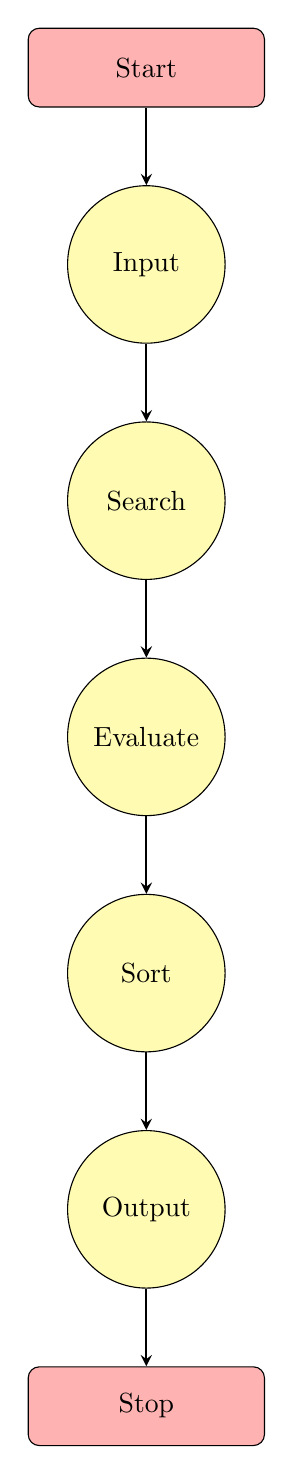
\begin{tikzpicture}[node distance=2cm]

        \node (start) [startstop] {Start};
        \node (func1) [function, below of=start, yshift=-0.5cm] {Input};
        \node (func2) [function, below of=func1, yshift=-1cm] {Search};
        \node (func3) [function, below of=func2, yshift=-1cm] {Evaluate};
        \node (func4) [function, below of=func3, yshift=-1cm] {Sort};
        \node (func5) [function, below of=func4, yshift=-1cm] {Output};
        \node (stop)  [startstop, below of=func5, yshift=-0.5cm] {Stop};

        \draw [arrow] (start) -- (func1);
        \draw [arrow] (func1) -- (func2);
        \draw [arrow] (func2) -- (func3);
        \draw [arrow] (func3) -- (func4);
        \draw [arrow] (func4) -- (func5);
        \draw [arrow] (func5) -- (stop);

    \end{tikzpicture}
\end{center}

%-----------------------------------------------------------------------------------------------------------------------

\newpage
\subsection{Input}
\noindent
\begin{center}
    \begin{tikzpicture}[node distance=2cm]

        \node (start) [startstop] {Start};
        \node (in1)  [io, below of=start] {Read start and end destination};
        \node (in2)  [io, below of=in1] {Read time of departure / arrival};
        \node (in3)  [io, below of=in2, text width=4cm, yshift=-1cm] {Read user choice:\\set preferences (Y)\\no
        preferences (N)\\ open custom file (F)};
        \node (dec1) [decision, below of=in3, yshift=-2cm] {Check choice};
        \node (pro1) [process, left of=dec1, xshift=-2.5cm] {Set preferences according to the file};
        \node (in4)  [io, right of=in1, xshift=4cm] {Read transport selection};
        \node (dec2) [decision, below of=in4, yshift=-1cm] {Car selected?};
        \node (in5)  [io, below of=dec2, yshift=-1cm] {Read fuel efficiency};
        \node (in6)  [io, below of=in5] {Read the priorities};
        \node (dec3) [decision, below of=in6, yshift=-1cm] {Save?};
        \node (pro2) [process, below of=dec3, yshift=-1cm] {Save current preferences to a file};
        \node (stop) [return, below of=dec1, text width=5cm, yshift=-3cm] {Return(start-id, dest-id, time, priorities, preferences, fuel)};

        \coordinate [right of=dec1, xshift=1cm] (ph1);
        \coordinate [left of=dec3, xshift=-0.5cm] (ph2);
        \coordinate [below of=ph2, yshift=-1cm] (ph3);
        \coordinate [right of=dec2, xshift=1cm] (ph4);

        \draw [arrow] (start) -- (in1);
        \draw [arrow] (in1) -- (in2);
        \draw [arrow] (in2) -- (in3);
        \draw [arrow] (in3) -- (dec1);
        \draw [arrow] (dec1) -- node[anchor=south] {F} (pro1);
        \draw [arrow] (pro1) |- (stop);
        \draw [arrow] (dec1) -- node[anchor=east] {N} (stop);
        \draw [line]  (dec1) -- node[anchor=south] {Y} (ph1);
        \draw [arrow] (ph1) |- (in4);
        \draw [arrow] (in4) -- (dec2);
        \draw [arrow] (dec2) -- node[anchor=east] {yes} (in5);
        \draw [arrow] (in5) -- (in6);
        \draw [line]  (dec2) -- node[anchor=south] {no} (ph4);
        \draw [arrow] (ph4) |- (in6);
        \draw [arrow] (in6) -- (dec3);
        \draw [line]  (dec3) -- node[anchor=south] {no} (ph2);
        \draw [line]  (ph2) -- (ph3);
        \draw [arrow] (dec3) -- node[anchor=east] {yes} (pro2);
        \draw [arrow] (pro2) -- (stop);

    \end{tikzpicture}
\end{center}

%-----------------------------------------------------------------------------------------------------------------------

\newpage
\begin{center}
    \begin{multicols}{3}
        \subsection{Search}
        \noindent
        \begin{tikzpicture}[node distance=2cm]

            \node (start) [return] {Start(start-id, dest-id, time)};
            \node (pro1) [process, below of=start] {Call Rejseplanens API with the given input};
            \node (pro2) [process, below of=pro1] {Save all the results};
            \node (stop) [return, below of=pro2] {Return(results)};

            \draw [arrow] (start) -- (pro1);
            \draw [arrow] (pro1) -- (pro2);
            \draw [arrow] (pro2) -- (stop);

        \end{tikzpicture}

        \vspace{2cm}

%-----------------------------------------------------------------------------------------------------------------------

        \subsection{Evaluate}
        \noindent
        \begin{tikzpicture}[node distance=2cm]

            \node (start) [return] {Start(results, prefrences, fuel)};
            \node (pro1) [process, below of=start] {Calculate attributes for each route};
            \node (pro2) [process, below of=pro1] {Evaluate routes using user's preferences};
            \node (pro3) [process, below of=pro2] {Add a numerical rating to each route};
            \node (stop) [return, below of=pro3] {Return(routes)};

            \draw [arrow] (start) -- (pro1);
            \draw [arrow] (pro1) -- (pro2);
            \draw [arrow] (pro2) -- (pro3);
            \draw [arrow] (pro3) -- (stop);

        \end{tikzpicture}

%-----------------------------------------------------------------------------------------------------------------------

        \subsection{Sort}
        \noindent
        \begin{tikzpicture}[node distance=2cm]

            \node (start) [return] {Start(routes, priorities)};
            \node (pro1) [process, below of=start] {Qsort the list of routes by user's priorities};
            \node (stop) [return, below of=pro1] {Return(routes)};

            \draw [arrow] (start) -- (pro1);
            \draw [arrow] (pro1) -- (stop);

        \end{tikzpicture}
    \end{multicols}
\end{center}

%-----------------------------------------------------------------------------------------------------------------------

\newpage
\subsection{Output}
\noindent
\begin{center}
    \begin{tikzpicture}[node distance=2cm]

        \node (start) [return] {Start(routes)};
        \node (out1)  [io, below of=start] {Print search results};
        \node (in1)   [io, below of=out1, text width=4cm, yshift=-0.5cm] {Read user choice:\\ view route details (1-5)\\
        sort the list (P,T,S,C)};
        \node (dec1)  [decision, below of=in1, yshift=-1.5cm] {Check int/char};
        \node (pro1)  [process, left of=dec1, xshift=-2.5cm] {Sort the list according to the input character};
        \node (func1) [function, below of=pro1, yshift=-1cm] {Sort};
        \node (out2)  [io, right of=dec1, xshift=2.5cm] {Print details for chosen route};
        \node (in2)   [io, below of=out2, text width=4cm, yshift=-0.5cm] {Read user choice:\\ go back to list (B)\\ quit
        the program (Q)};
        \node (dec2)  [decision, below of=in2, yshift=-1.5cm] {Check choice};
        \node (stop)  [startstop, left of=dec2, xshift=-2.5cm] {Stop};

        \coordinate [right of=dec2, xshift=1.5cm] (ph1);

        \draw [arrow] (start) -- (out1);
        \draw [arrow] (out1) -- (in1);
        \draw [arrow] (in1) -- (dec1);
        \draw [arrow] (dec1) -- node[anchor=south] {char} (pro1);
        \draw [arrow] (pro1) -- (func1);
        \draw [arrow] (dec1) -- node[anchor=south] {int} (out2);
        \draw [arrow] (out2) -- (in2);
        \draw [arrow] (in2) -- (dec2);
        \draw [arrow] (dec2) -- node[anchor=south] {Q} (stop);
        \draw [line] (dec2) -- node[anchor=south] {B} (ph1);
        \draw [arrow] (ph1) |- (out1);

    \end{tikzpicture}
\end{center}

%-----------------------------------------------------------------------------------------------------------------------
% textidote: ignore end

\section{Calculating the attributes}

Before we can properly print results in the program, we need to calculate the attributes of the different routes.
This is a relatively difficult task, as we need to calculate the distance, price, \unit{CO_{2}} and comfort.
Some attributes are easier to calculate than others, but they all require some form of calculation.

Rejseplanen has systems in place to calculate some of those attributes, but the API does not provide them.
This means that we have to calculate them ourselves.
Our calculations will not be 100\% accurate, but they will be close enough for our purposes.

\subsection{Calculating distance}

As we don't use a map API, we can't properly calculate the distance between two points.
This means that we have to ignore roads and instead calculate the distance by the train tracks.
The problem is that Rejseplanen only provides the coordinates of the stations, not the tracks.
So what we decided to do instead is to calculate the distance between the stations.
This won't account for curves along the track, as the distance is calculated as a straight line between the stations.
However, doing this for every station along the route is better than doing this for only the start and end station.

\begin{figure}[H]
    \centering
    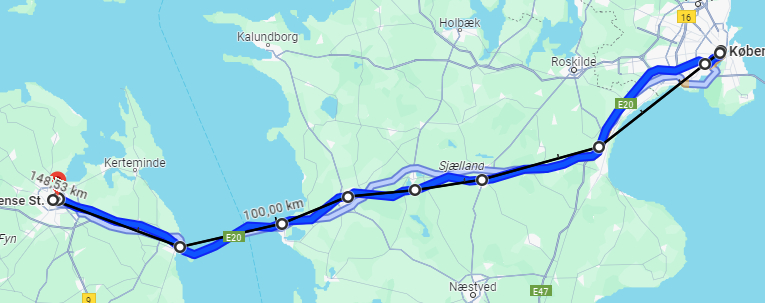
\includegraphics[width=0.8\textwidth]{images/google-maps-distance-calculation.jpg}
    \caption{A route between Copenhagen and Odense. \\ Blue line is Google Maps' distance, black line is our distance}
\end{figure}

% TODO Add explanation for how we calculate the distance

\subsection{Calculating price}

Calculating the price is a lot more difficult than calculating the distance.
As Denmark is divided into zones, the price is calculated based on how many zones you travel through.
The price is also affected based on a number of different variables, such as age, region, occupation and more.
For our program, we decided to calculate the prices for Pendlerkort and Ungdomskort.

\subsubsection{Zones}

First thing we need to do is to figure out how many zones a route goes through.
Unfortunately, Rejseplanen's API does not provide any information about how many zones a route goes through.
What we decided to do instead is to find the average size for a zone.
As the zones are not all the same size, the number of zones a route passes through may be slightly off.
But this is the best we can do with the current circumstances.

First we started by picking two stations and counted how many zones the route goes through using DSB's zone map. % cite here https://www.dsb.dk/globalassets/pdf/trafikinformation/storezoner-22.pdf
We then used Google Maps to calculate the distance along the tracks between two stations and we noted it down.
Finally we divided the distance by the number of zones to get the average size of a zone along the route.

\begin{figure}[H]
    \centering
    \noindent
    \begin{tabular}{ || c | c | c || }
        \hline
        Route & Zones and distance & Zone size \\
        \hline\hline
        Korsør to Ringsted & 5 zones 45 km & 9 km per zone \\
        \hline
        Ringsted to Køge Nord & 6 zones 30 km & 5 km per zone \\
        \hline
        Kalundborg to Holbæk & 7 zones 45 km & 6.4 km per zone \\
        \hline
        Frederikssund to Kbh & 10 zones 23 km & 2.3 km per zone \\
        \hline
        Voldingborg to Ringsted & 8 zones 52 km & 6.5 km per zone \\
        \hline\hline
        Zone Averages & & 6 km per zone \\
        \hline
    \end{tabular}
    \caption{Table of our calculations of zone size averages}
\end{figure}

We determined that the average size of a zone is roughly about 6 kilometers.
But as you can see, the sizes of zones varies a lot.
This is unfortunate for us, as it means that the number of zones a route goes through may be very inaccurate.

\subsubsection{Pendlerkort price}

The way we're goint to calculate the price will is by figuring out the price for Pendlerkort.
This card allows commuters to freely travel between set amount of zones.
Rejseplanen has a website where the user can input their route and it'll calculate the price for the Pendlerkort. % cite here https://www.rejseplanen.dk/bin/query.exe/mn?L=vs_rkfc
We then took the results and compared them to the price chart provided by DSB. % cite here https://www.dsb.dk/globalassets/priser_og_zoner/2023/000000_priser_rabatter_jylland_fyn_a4_15_jan23.pdf
The results are accurate enough that we deemed them good enough for our purposes.

\begin{figure}[H]
    \centering
    \noindent
    \begin{tabular}{ || c | c || }
        \hline
        Route & Zones and price \\
        \hline\hline
        Odense to København & 30 zones 3750 kr \\
        \hline
        Køge Nord to København & 9 zones 1470 kr \\
        \hline
        Græsted to Vordingborg & 18 zones 3000 kr \\
        \hline
        Aarhus to København & 51 zones 4590 kr \\
        \hline
    \end{tabular}
    \caption{Table of Rejseplanen's price calculations}
\end{figure}

\begin{figure}[H]
    \centering
    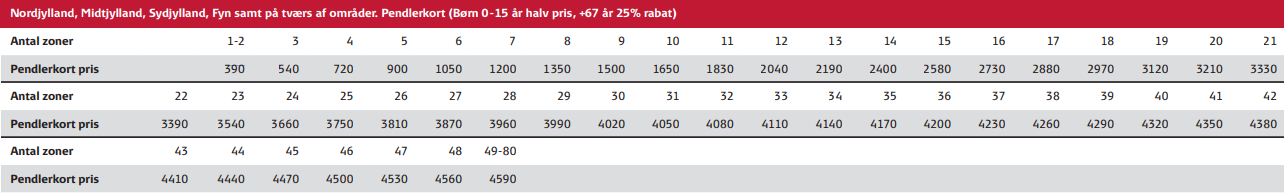
\includegraphics[width=1\textwidth]{images/dsb-pendlerkort-pris.jpg}
    \caption{Price of Pendlerkort per zones}
\end{figure}

From what it seems, the price table is not recursive, so we can't implement a recursive function to calculate the price.
Instead, we can save the table in the program and reference it when we need to find the price.
This allows us to have a pretty accurate price chart as long as the number of zones is accurate.

\subsubsection{Ungdomskort price}

Ungdomskort is a type op Pendlerkort that is primarily aimed at young people or students.
The price is significantly lower than Pendlerkort, so we deemed it necessary to implement it in our program.
Calculating the price for Ungdomskort is a lot easier than Pendlerkort, as the method is listed on their website. % cite here https://www.ungdomskort.dk/priser/

The price is calculated by taking the equivalent price for a Pendlerkort and then taking 2487 kr from it.
Then the result is halved and you add 663 kr to the result.
Here's an example for a Pendlerkort that costs 3750 kr:

\begin{equation}
    \frac{3750 - 2487}{2} + 663 = 1294 kr
\end{equation}

As a member in our group travels with Ungdomskort, we can confirm that this result is accurate.

% textidote: ignore begin
\subsection{Calculating \unit{CO_{2}} emission}
% TODO Add the calculations, remove textiodte ignore
% textidote: ignore end

% textidote: ignore begin
\subsection{Calculating comfort value}
% TODO Add the calculation, remove textiodte ignore
% textidote: ignore end

\section{Saving user preferences}\label{sec:saving-user-preferences}

To make our program more user-friendly, we want to be able to store a users preferences on climate, price,
time, and so on.
This will be stored locally in a configuration file, which we will call
``\verb|preferences.json|''.
As the name suggests we have chosen to store the data in a JSON format, this is partly because we already have
a system in place in order to store JSON data, but also because it allows us to access individual keys of data such as
``price''.
If implemented correctly storing the preferences as JSON also allows us to remove or add different keys to the file
later if it is needed, but at this point we only need to save four keys called: price, time, environment and health.

For the actual implementation for saving the file.
We will, if the program is executed, always require data for all our chosen preference categories.
A way to do this is to, at the programs start, initialize the save file with some standard data, so the program can
continue running even if the user does not want to input their own preferences.
We initialize the save file through a function called ``InitializePreferenceFile''

\begin{lstlisting}[label={lst:SavePreferences}, caption={Saving preferences to file.}]
    FILE* preferences = fopen("preferences.json", "w");
    fputs(kSerializedJsonWithNewline, preferences);
    fclose(preferences);
    free(kSerializedJsonWithNewline);

    cJSON_Delete(kJsonPreferences);
\end{lstlisting}

In Figure~\ref{lst:SavePreferences} it can be seen that we are trying to open the preferences file,
and by using ``fopen'' we make use of the property that creates the file if it does not already exist.
The rest of the code inside InitializePreferenceFile is used to convert our given inputs into the JSON format, which in
C is somewhat difficult.

The remaining functions for the preference file are SetUserPreference and GetUserPreference.
The SetUserPreference function will work by taking in two inputs, a key and a value for that key.
This would be written as \(SetUserPreference("key", value)\).
When we want to change the values in the JSON file through C, we must first read the file and then parse it as cJSON[.]
In this way we can actually make the changes to the stored values.
Parsing JSON and generating JSON is done through the library cJSON which we have chosen to use.
As seen above it works by first parsing the content of the preference file and then searching for the item we want to
change.

\begin{lstlisting}[label={lst:ParseJSON}, caption={Parsing JSON.}]
  const cJSON* const kJsonPreferences = cJSON_Parse(kFileBuffer);
  free(kFileBuffer);

  cJSON* const kJsonValue = cJSON_GetObjectItem(kJsonPreferences, key);

  kJsonValue->valuedouble = value;
\end{lstlisting}

cJSON stores all JSON values as structs and to change the value we access the struct as seen on line 82 in
Figure~\ref{lst:ParseJSON}.
The next step is then to save the changes to our preferences file, but because saving to a file in C can get
complicated if you change the length of the file, we sidestep this problem by overwriting the whole save file with the
updated values.

Finally, the last step is to read the file, so we can use the stored data in our program.
This is done much in the same way we used in SetUserPreference as we open the file, parse the JSON and then access
the item we want to use.
Both InitializePreferenceFile and SetUserPreference are void functions, but GetUserPreference is a double function
this is done so the returned value will be the value for the preference we want to get out of the save file, see
Figure~\ref{lst:GetPref}.
GetUserPreference only takes in one input which is the key we want to look for, this could be ``price'' or another of
the attributes.

\begin{lstlisting}[label={lst:GetPref}, caption={Reading attribute value from preference file.}]
  cJSON* file_item = cJSON_GetObjectItem(json_preferences, key);

  value = cJSON_GetNumberValue(file_item);

  cJSON_Delete(json_preferences);

  return value;
\end{lstlisting}

With these three functions it is now possible for us to store and use preferences locally on the device.

% textidote: ignore begin
\section{Evaluating the attributes}\label{sec:evaluating-the-attributes}
% textidote: ignore end

After the attributes for each route has been calculated, the attributes are evaluated against each other, as stated in
the flowchart.
To perform these comparisons the \texttt{Evaluate} function, as seen in~\ref{lst:evaluate-prototype}, is used.

\begin{lstlisting}[caption={Function prototype for \texttt{Evaluate}}, label={lst:evaluate-prototype}]
void Evaluate(TripData trip_arr[], size_t size_of_struct_array);
\end{lstlisting}

This routine has an array of the type \texttt{TripData} as an input parameter, which is a struct type as seen in
~\ref{lst:TripData-declaration}.

\begin{lstlisting}[caption={Declaration of \texttt{TripData} struct}, label={lst:TripData-declaration}]
typedef struct TripData {
  int trip_id;
  double price;
  double comfortability;
  double time;
  double emissions;
} TripData;
\end{lstlisting}

This, as well as the size of the array, allows the \texttt{Evaluate} function to read from the members served by the
\texttt{Calculating} functions mentioned earlier as well as write to the \texttt{\_score} members.
This function's primary function is to call the function \texttt{CalculateScore} function, as seen in
~\ref{lst:calculatescore-prototype}, with the different attributes of the routes as input parameters.

\begin{lstlisting}[caption={Function prototype for \texttt{CalculateScore}}, label={lst:calculatescore-prototype}]
void CalculateScore(TripData trip_data[], const CalculateScoreParameters* calculate_score_parameters);
\end{lstlisting}

It does this by having the struct array mentioned before and by having an instance of the
\texttt{CalculateScoreParameters} struct, as seen in~\ref{lst:CalculateScoreParameters-declaration} as input parameters.

\begin{lstlisting}[caption={Declaration of \texttt{CalculateScoreParameters} struct},
    label={lst:CalculateScoreParameters-declaration}]
typedef struct CalculateScoreParameters {
  const size_t kNumTrips;
  const size_t kReadOffset;
  const size_t kWriteOffset;
  const int kInverted;
} CalculateScoreParameters;
\end{lstlisting}

This struct is used to pass multiple input parameters without clouding the input parameters of the function.
The functionality of the \texttt{CalculateScore} function includes identifying the largest and smallest member of a
specific member type for all iterations of the struct array.
The initialization of the local variable \texttt{Score}, as seen in~\ref{lst:score_initialization}, includes the score
calculation for each instance of the struct for the relevant member passed in the \texttt{CalculateScore} function.

\begin{lstlisting}[caption={Initialization of \texttt{Score}}, label={lst:score_initialization}]
double score = (*(double*)read_member - attribute_smallest) /
  (attribute_largest - attribute_smallest);
\end{lstlisting}

By subtracting the smallest member from the value of each member, as well as the largest member, the values are shifted
to a common baseline of \texttt{0}.
The score for the relevant member for each route is then given relative to the largest and smallest member, hereby
given one member the score of \texttt{1}, another the score of \texttt{0} and the rest the relative score in between.

This process is as mentioned iterated over all member types in the \texttt{TripData} struct array.

Finally, the \texttt{overall\_score} member is calculated for all the iterations in the struct array, as seen in
~\ref{lst:overall_score-calculation}.

\begin{lstlisting}[caption={Calculation of \texttt{overall\_score}}, label={lst:overall_score-calculation}]
for (size_t i = 0; i < size_of_struct_array; i++) {
  trip_arr[i].overall_score =
      GetUserPreference("price") * trip_arr[i].price_score +
      GetUserPreference("health") * trip_arr[i].comfortability_score +
      GetUserPreference("time") * trip_arr[i].time_score +
      GetUserPreference("environment") * trip_arr[i].emissions_score;
}
\end{lstlisting}







    \bibliographystyle{IEEEtran}
    \bibliography{problem-analysis/audience,problem-analysis/existing-solutions,problem-analysis/financial-awareness,problem-analysis/history,problem-analysis/what-is-the-problem}
\end{document}
